%%%%%%%%%%%%%%%%%%%%%%%%%%%%%%%%%%%%%%%%%
% Beamer Presentation
% LaTeX Template
% Version 1.0 (10/11/12)
%
% This template has been downloaded from:
% http://www.LaTeXTemplates.com
%
% License:
% CC BY-NC-SA 3.0 (http://creativecommons.org/licenses/by-nc-sa/3.0/)
%
%%%%%%%%%%%%%%%%%%%%%%%%%%%%%%%%%%%%%%%%%

%----------------------------------------------------------------------------------------
%	PACKAGES AND THEMES
%----------------------------------------------------------------------------------------

\documentclass{beamer}

\mode<presentation> {

% The Beamer class comes with a number of default slide themes
% which change the colors and layouts of slides. Below this is a list
% of all the themes, uncomment each in turn to see what they look like.

%\usetheme{default}
%\usetheme{AnnArbor}
%\usetheme{Antibes}
%\usetheme{Bergen}
%\usetheme{Berkeley}
%\usetheme{Berlin}
%\usetheme{Boadilla}
%\usetheme{CambridgeUS}
%\usetheme{Copenhagen}
%\usetheme{Darmstadt}
%\usetheme{Dresden}
%\usetheme{Frankfurt}
%\usetheme{Goettingen}
%\usetheme{Hannover}
%\usetheme{Ilmenau}
%\usetheme{JuanLesPins}
%\usetheme{Luebeck}
\usetheme{Madrid}
%\usetheme{Malmoe}
%\usetheme{Marburg}
%\usetheme{Montpellier}
%\usetheme{PaloAlto}
%\usetheme{Pittsburgh}
%\usetheme{Rochester}
%\usetheme{Singapore}
%\usetheme{Szeged}
%\usetheme{Warsaw}

% As well as themes, the Beamer class has a number of color themes
% for any slide theme. Uncomment each of these in turn to see how it
% changes the colors of your current slide theme.

%\usecolortheme{albatross}
%\usecolortheme{beaver}
%\usecolortheme{beetle}
%\usecolortheme{crane}
%\usecolortheme{dolphin}
%\usecolortheme{dove}
%\usecolortheme{fly}
%\usecolortheme{lily}
%\usecolortheme{orchid}
%\usecolortheme{rose}
%\usecolortheme{seagull}
%\usecolortheme{seahorse}
%\usecolortheme{whale}
%\usecolortheme{wolverine}

%\setbeamertemplate{footline} % To remove the footer line in all slides uncomment this line
%\setbeamertemplate{footline}[page number] % To replace the footer line in all slides with a simple slide count uncomment this line

%\setbeamertemplate{navigation symbols}{} % To remove the navigation symbols from the bottom of all slides uncomment this line
}

\usepackage{graphicx} % Allows including images
\usepackage{booktabs} % Allows the use of \toprule, \midrule and \bottomrule in tables
\usepackage{rotating}

%----------------------------------------------------------------------------------------
%	TITLE PAGE
%----------------------------------------------------------------------------------------

\title[Spatial Interpolation. Summer Academy `15]{Spatial(-temporal) Interpolation with R\\
\medskip \tiny{International Summer Academy on Spatial Ecotoxicology and Ecotoxicological Risk Assessment\\Using an Open Commmunity Approach}} % The short title appears at the bottom of every slide, the full title is only on the title page

\author[Avit Bhowmik]{Avit Kumar Bhowmik \\} % Your name
\institute[Uni Koblenz-Landau] % Your institution as it will appear on the bottom of every slide, may be shorthand to save space
{
Institute for Environmental Sciences, University of Koblenz-Landau \\ % Your institution for the title page
\medskip
\textit{bhowmik@uni-landau.de}% Your email address
}
\date{\today} % Date, can be changed to a custom date

\begin{document}

\begin{frame}
\titlepage % Print the title page as the first slide
\end{frame}

%------------------------------------------------

\begin{frame}
\frametitle{What do we know?}
\centering
\Huge \alert{What is GIS?}\\
\vspace{1cm}

\includegraphics[width=0.4\textwidth]{Figures/Questions.png}
\end{frame}

%------------------------------------------------

\begin{frame}
\centering
\Huge \alert{\textbf{GIS}}\\
\pause
\Large \textbf{? Information ?}
\pause
\medskip
\normalsize
\begin{columns}[t]
\column{.6\textwidth}
\begin{itemize}
\item \alert{\textbf{Geographic}}\\
Parent and Church, 1987. Conf. GIS
\item \alert {\textbf {Spatial (Geospatial)}}\\
Anselin, 1989. What is special about spatial data?
\item \alert{\textbf{Spatiotemporal}}\\
Burrough and Frank, 1995. Int J GIS
\end{itemize}
\hspace{2cm}
\pause
\column{.5\textwidth}
\begin{itemize}
\item \alert{\textbf{System}}
\item \alert{\textbf{Science}}\\
Goodchild, 1992. Int J GIS
\end{itemize}
\end{columns}
\end{frame}

%------------------------------------------------

\begin{frame}
\frametitle{80\% of data are Spatiotemporal}
\centering
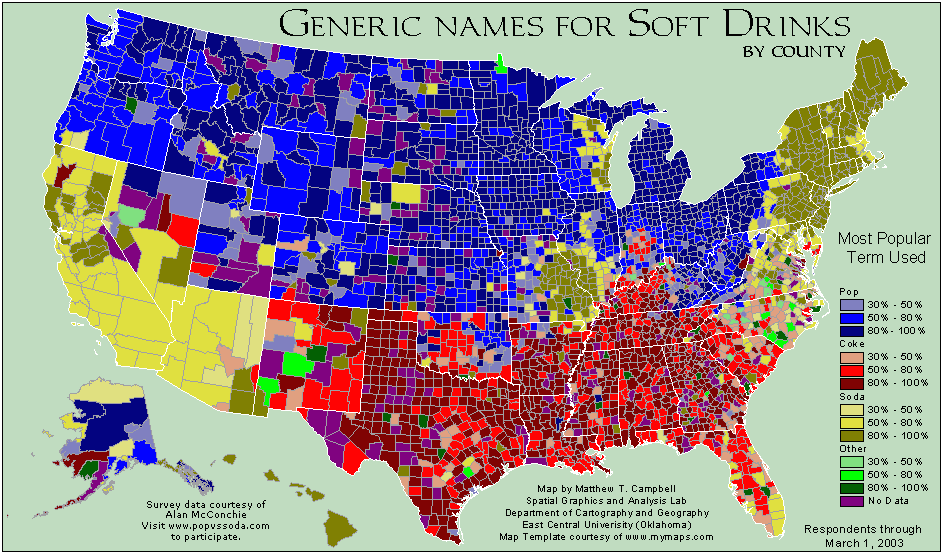
\includegraphics[width=0.9\textwidth]{Figures/softdrinks.png}\\
Bossler, 2002. Manual of Geospatial Science and Technology
\end{frame}

%-----------------------------------------------

\begin{frame}
\frametitle{Representation of Spatiotemporal Data}
\centering
\onslide<2->\begin{turn}{90}
\begin{minipage}[c]{6cm}
\centering
\hspace{0.8cm} Time\\\hspace{0.8cm} (Step or Interval or Series)
\end{minipage}
\end{turn}
\onslide<1->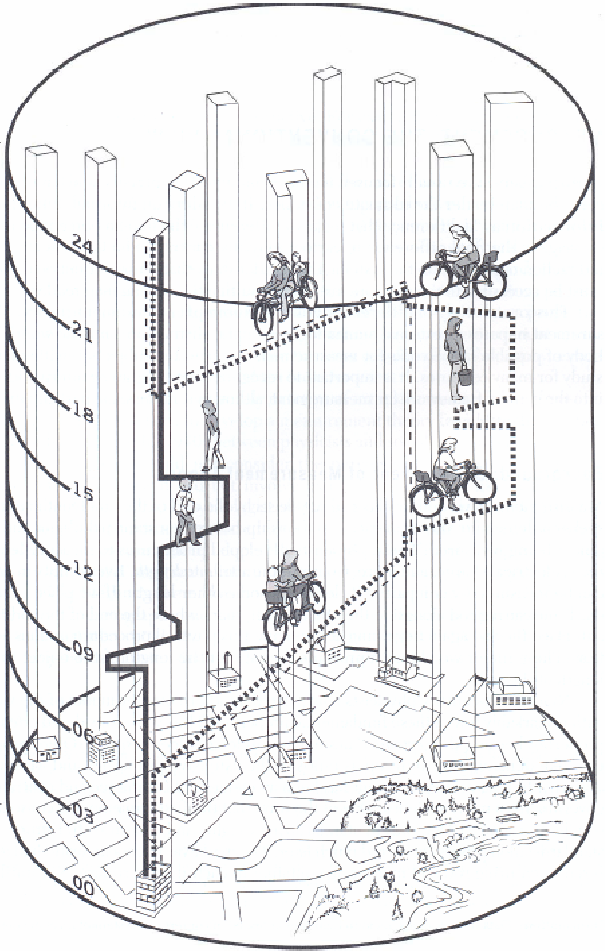
\includegraphics[width=0.38\textwidth]{Figures/RepGI.png} \hspace{1cm} \alert{\footnotesize Chrisman,1997.Exploring GIS}\\
\onslide<2->\hspace{-3.5cm} Space (x,y)
\end{frame}

%-----------------------------------------------

\begin{frame}
\frametitle{Wear the GI Glasses}
\centering

\includegraphics[width=0.7\textwidth]{Figures/GIglass.png}
\end{frame}

%------------------------------------------------

\begin{frame}
\frametitle{What do we know?}
\centering
\Huge \alert{What is Spatial Statistics?}\\
\vspace{1cm}

\includegraphics[width=0.4\textwidth]{Figures/Questions.png}
\end{frame}

%------------------------------------------------

\begin{frame}
\frametitle{Spatial(-temporal) Statistics}
\begin{block}{Experts’ Thoughts}
\begin{itemize}
\item Spatial statistics offers a way of describing the spatial continuity that is an essential feature of many natural phenomena and provides adaptations of classical regression techniques to take the advantage of this continuity\\
\small \alert{Isaaks and Srivastava, 1989. An Introduction to Applied Geostatistics}
\normalsize
\vspace{1cm}
\item Spatial statistics provides a set of statistical tools for incorporating the spatial coordinates of observations in data processing\\
\small \alert{Goovaerts, 2007. Geostatistics for Natural Resources Evaluation}
\end{itemize}
\end{block}
\end{frame}

%-----------------------------------------------

\begin{frame}
\frametitle{Spatial(-temporal) Interpolation}
\centering
$\vcenter{\hbox{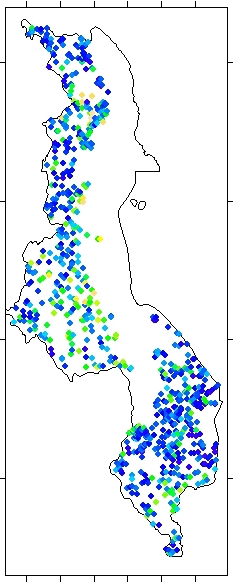
\includegraphics[width=0.24\textwidth]{Figures/Mwipt.png}}}$
\hspace{1cm} \onslide<2-> \Huge \alert{z} \hspace{1cm}
\onslide<1->$\vcenter{\hbox{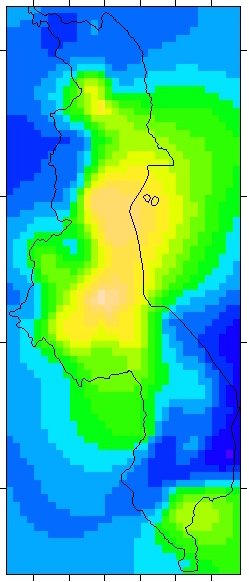
\includegraphics[width=0.25\textwidth]{Figures/Mwisf.png}}}$\\
\onslide<2->
\small
\alert{z is a random process with unique mean and variance}\\
\alert{z(sampled locations) $\approx$ z(unsampled location)}
\end{frame}

%-----------------------------------------------

\begin{frame}
\frametitle{Spatial(-temporal) Interpolation}
\begin{block}{Input}
\begin{itemize}
\item  Set of Points sampled, sparsely distributed in space and time
\item  Each point represents a measurement of a variable (spatiotemporal attribute) that occurs in that space and time location
\end{itemize}
\end{block}
\vspace{1 cm}
\pause
\begin{block}{Output}
\begin{itemize}
\item \alert{Spatial Data Model}
\item Computer/mathematical representation that allows one to perform estimations and/or simulations for attribute values at spatial/temporal locations not sampled
\end{itemize}
\end{block}
\end{frame}

%------------------------------------------------

\begin{frame}
\frametitle{Spatial(-temporal) Variability}
\centering
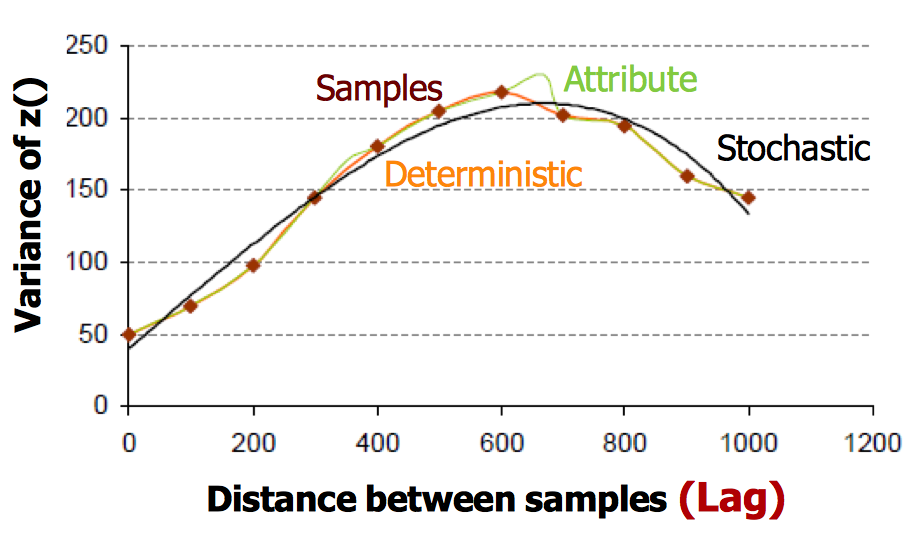
\includegraphics[width=\textwidth]{Figures/vario.png}
\end{frame}

%------------------------------------------------

\begin{frame}
\frametitle{Spatial(-temporal) Variability}
\centering
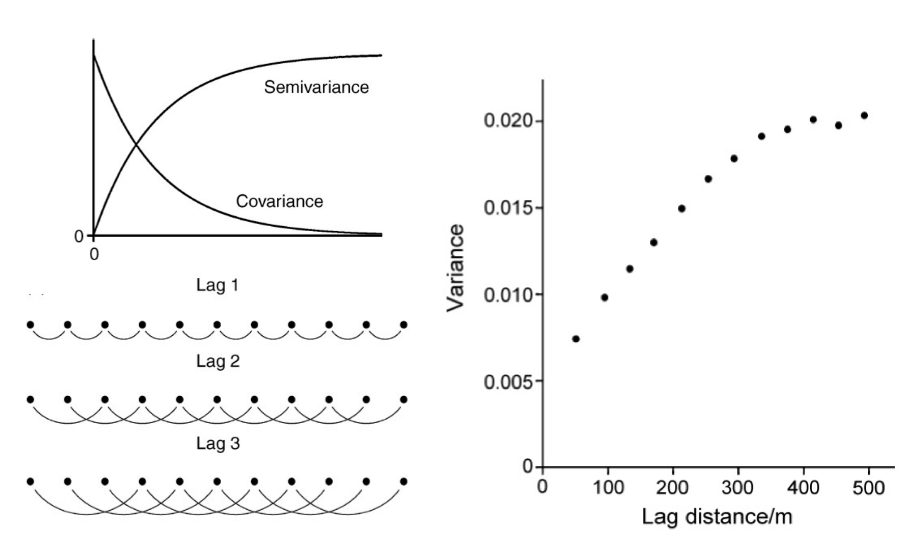
\includegraphics[width=\textwidth]{Figures/vario1.png}
\end{frame}

%------------------------------------------------

\begin{frame}
\frametitle{Spatial(-temporal) Variogram}
\centering
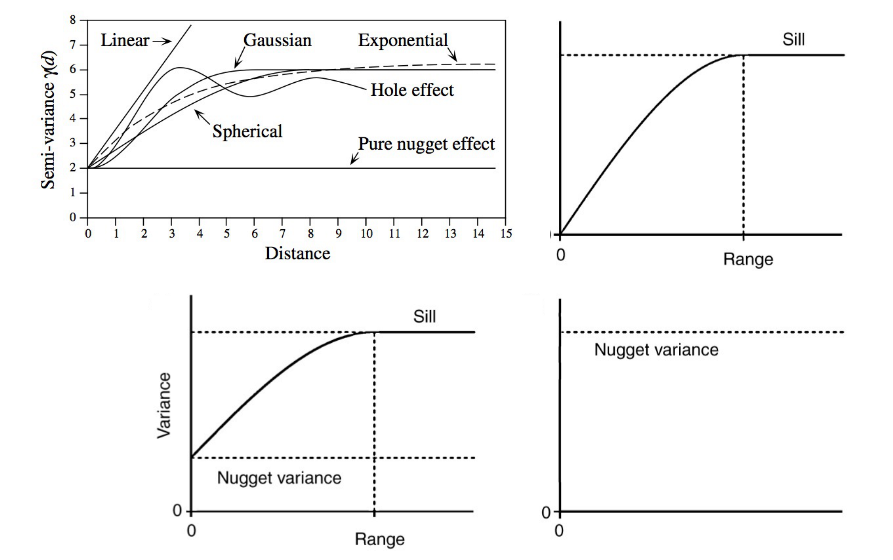
\includegraphics[width=\textwidth]{Figures/variogram.png}
\end{frame}

%------------------------------------------------

\begin{frame}
\frametitle{Stochastic or Geostatistical Interpolation}
\begin{itemize}
\item A probability distribution function is associated to its probable values
\item Uncertainties can be associated to its estimation
\item \alert{e.g. Kriging}
\item \alert{Minimization of estimation variance (error)}
\end{itemize}
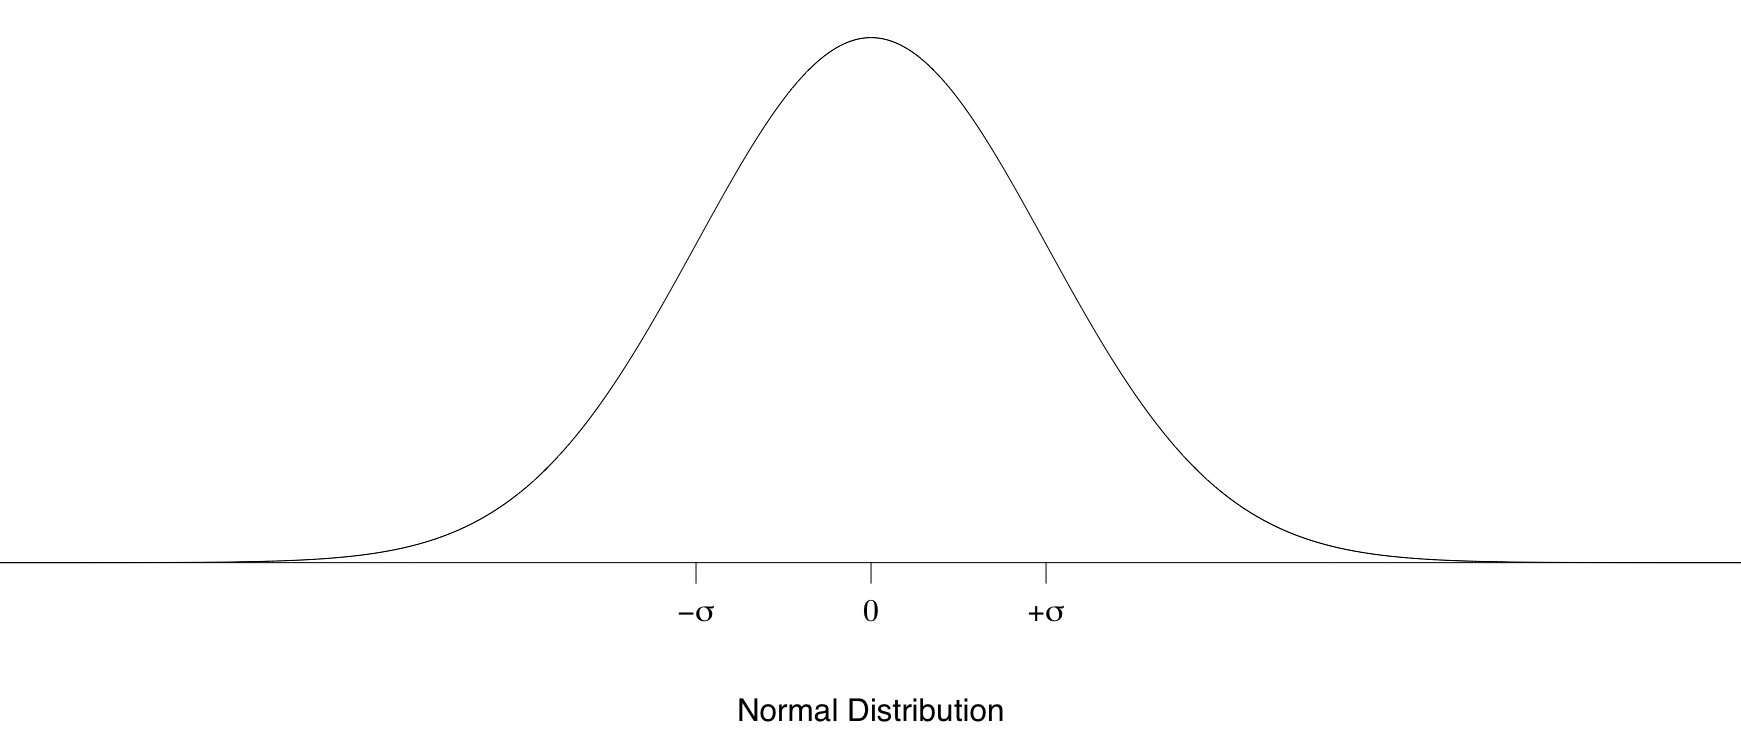
\includegraphics[width=0.8\textwidth]{Figures/normald.png}
\end{frame}

%------------------------------------------------

\begin{frame}
\frametitle{Deterministic Interpolation}
\begin{itemize}
\item An unique value is associated to its spatial location
\item No uncertainty is associated to its estimation
\item \alert{e.g. Inverse Distance Weighting (IDW)}
\end{itemize}
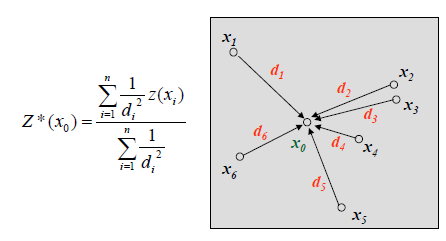
\includegraphics[width=0.7\textwidth]{Figures/idw.png}
\end{frame}

%------------------------------------------------

\begin{frame}
\frametitle{Learn more about Spatial(-temporal) Statistics}
\centering
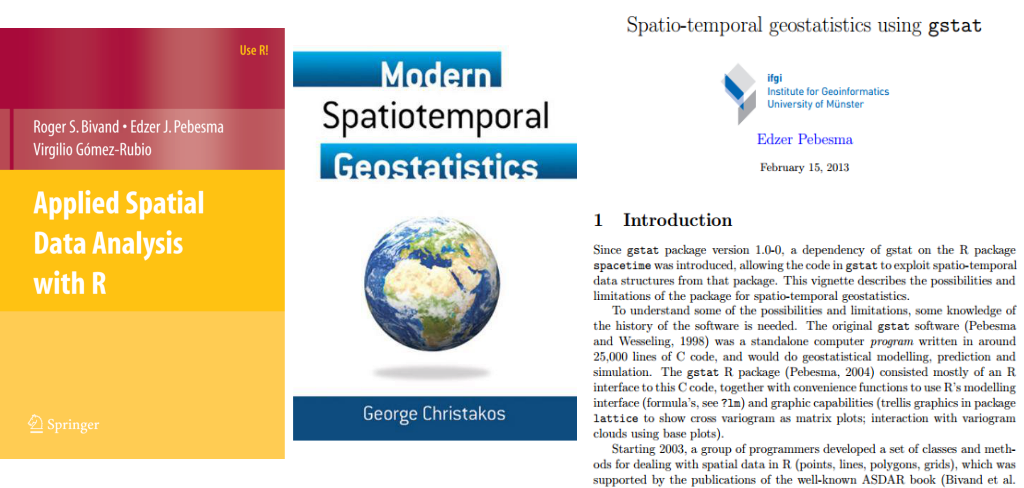
\includegraphics[width=\textwidth]{Figures/books.png}
\end{frame}

%------------------------------------------------

\begin{frame}
\frametitle{Learn more about Spatial(-temporal) Statistics}
\centering
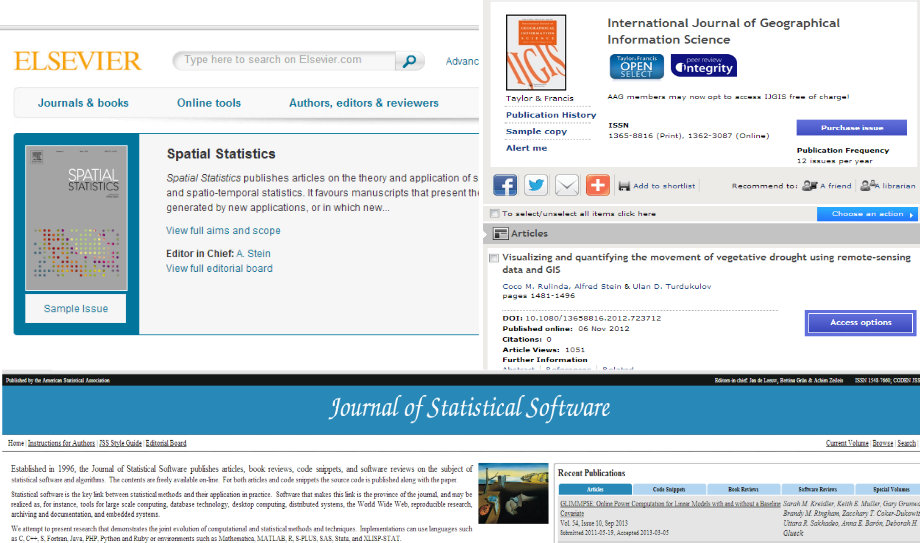
\includegraphics[width=\textwidth]{Figures/journals.png}
\end{frame}

%------------------------------------------------

\begin{frame}
\centering
The slides, scripts, materials and data are available from:\\
\href{https://github.com/AvitBhowmik/summer_academy_15}{\alert{https://github.com/AvitBhowmik/summer\textunderscore academy\textunderscore 15}}\\
\vspace{1cm}
\Huge Thank You!
\end{frame}

%------------------------------------------------

\end{document} 